\documentclass[10pt,a4paper]{article}

% --- Layout ---
\usepackage[margin=2cm, top=2.5cm]{geometry}
\usepackage{parskip}
\usepackage{microtype}

% --- Math ---
\usepackage{amsmath, amssymb}

% --- Tables ---
\usepackage{booktabs}
\usepackage{array}
\usepackage{tabularx}
\usepackage{multirow}

% --- Graphics ---
\usepackage{graphicx}
\usepackage{float}

% --- Sections ---
\usepackage{titlesec}
\titleformat{\section}{\large\bfseries}{}{0em}{}[\titlerule]
\titleformat{\subsection}{\normalsize\bfseries}{}{0em}{}
\titlespacing{\section}{0pt}{1.4ex plus .2ex}{0.5ex}
\titlespacing{\subsection}{0pt}{0.9ex}{0.3ex}

% --- Lists ---
\usepackage{enumitem}
\setlist{noitemsep, topsep=2pt, parsep=0pt}

% --- Colours and links ---
\usepackage{xcolor}
\definecolor{linkblue}{rgb}{0.08,0.18,0.55}
\definecolor{midgray}{gray}{0.40}
\definecolor{flagred}{rgb}{0.72,0.11,0.11}
\definecolor{passgreen}{rgb}{0.13,0.55,0.13}
\definecolor{warnamber}{rgb}{0.80,0.50,0.00}
\definecolor{mmp2blue}{rgb}{0.28,0.47,0.81}
\definecolor{mmp9green}{rgb}{0.42,0.80,0.40}
\definecolor{nered}{rgb}{0.84,0.37,0.37}
\usepackage{hyperref}
\hypersetup{colorlinks=true, urlcolor=linkblue, linkcolor=black, citecolor=midgray}

% --- tcolorbox for callouts ---
\usepackage{tcolorbox}

% --- Header / Footer ---
\usepackage{fancyhdr}
\pagestyle{fancy}
\fancyhf{}
\lhead{\small\textbf{Dry Lab Deliverable: Task 8} \textbullet{} Eton iGEM 2026}
\rhead{\small Aaran Nihalani}
\cfoot{\small\thepage}
\renewcommand{\headrulewidth}{0.3pt}
\renewcommand{\footrulewidth}{0pt}

% --- Convenience macros ---
\newcommand{\kcat}{$k_{\text{cat}}/K_M$}
\newcommand{\MMP}[1]{\textbf{MMP-#1}}
\newcommand{\NE}{\textbf{NE}}
\newcommand{\seq}[1]{\texttt{#1}}
\newcommand{\kap}{$\kappa$}

\begin{document}

% ---------------------------------------------------------------------------
%  Title block
% ---------------------------------------------------------------------------
\begin{center}
  {\LARGE\bfseries 3-Plex Substrate Design}\\[0.15em]
  {\normalsize Task 8 \textbullet{} Dry Lab Deliverable}\\[0.08em]
  {\small Aaran Nihalani \textbullet{} Eton iGEM 2026 \textbullet{} \today}
\end{center}
\vspace{0.3em}\hrule\vspace{0.6em}

This report delivers three device-ready 8-mer peptide substrates for a multiplexed
electrochemical biosensor targeting the chronic-wound protease panel:
{\color{mmp2blue}\textbf{MMP-2}}, {\color{mmp9green}\textbf{MMP-9}},
and {\color{nered}\textbf{neutrophil elastase (NE)}}.
All candidates are literature-seeded and validated against the VHSE8 + logistic-regression
classifiers trained on MEROPS cleavage data. A new MMP-2 classifier (2{,}318 positives,
AUROC~0.883) was added to the pipeline. The PSSM-based condition number $\kappa = 98$ on the 3$\times$3 specificity matrix
signals a conservative warning about gelatinase channel separation; however, this
is a sequence-similarity proxy built on candidates that score atypically under their
own MEROPS-derived PSSMs, and is not a definitive verdict. Published differential
$k_{\text{cat}}/K_M$ data suggest 3--10$\times$ kinetic selectivity is achievable
between MMP-2 and MMP-9, which would give $\kappa(A_{\text{kin}}) \approx 5$--10.
\textbf{The 3-plex design is retained as the primary target};
the sfGFP cleavage screen is the decision gate that will determine the true
kinetic condition number and confirm or revise the channel architecture.

% ---------------------------------------------------------------------------
\section{Background and Clinical Motivation}
% ---------------------------------------------------------------------------

Chronic wounds affect $\sim$2\% of the Western population and account for
\$25 billion in annual US healthcare expenditure.
MMP-9 is the dominant protease in non-healing diabetic foot ulcer (DFU) wound fluid;
its activity level predicts healing outcome with AUC~$= 0.901$
(sensitivity 81.8\%, Jindatanmanusan et al.\ 2018).
Total MMP activity is $\sim$30$\times$ elevated in chronic versus acute wounds
(Trengove et al.\ 1999), and the MMP-9/TIMP-1 ratio is an independent prognostic
marker (Ladwig 2002). Neutrophil elastase (NE) is co-elevated in non-healing wounds
($>$100~nM; PMC5487915) and provides a mechanistically orthogonal serine-protease channel.

A threshold rule (\textit{``signal above X~nM $\Rightarrow$ non-healing''}) ignores
uncertainty in the measured concentration and the population-level nature of protease
elevation. The long-term goal is a Bayesian posterior
$P(\text{healing} \mid \text{activity fingerprint})$
that propagates sensor noise through a kinetic model to a calibrated disease probability.
This task delivers the three substrate sequences the wet lab needs to run the sfGFP
cleavage screen and ultimately the electrochemical assay.

% ---------------------------------------------------------------------------
\section{MMP-2 Classifier: New Training Data}
% ---------------------------------------------------------------------------

MMP-2 (MEROPS M10.003, gelatinase~A) was not in the Task~7 panel.
It was added for Task~8 because MMP-2 and MMP-9 are the dominant gelatinases in wound fluid
and both must be accounted for in the device channel model.

\begin{table}[H]
\centering
\begin{tabularx}{\textwidth}{@{}p{1.8cm} p{1.8cm}
  >{\raggedleft\arraybackslash}p{2.4cm}
  p{2.0cm} X@{}}
\toprule
\textbf{Protease} & \textbf{MEROPS ID} & \textbf{Positives} & \textbf{Confidence} & \textbf{Notes} \\
\midrule
MMP-2  & M10.003 & 2{,}318 & \textcolor{passgreen}{\textbf{high}} & New — gelatinase A; 72\% identity to MMP-9 \\
MMP-9  & M10.004 &    341  & \textcolor{passgreen}{\textbf{high}} & Existing \\
NE     & S01.131 &    327  & \textcolor{passgreen}{\textbf{high}} & Existing \\
\bottomrule
\end{tabularx}
\caption{3-plex training data. All three classifiers meet the high-confidence threshold
($\geq$200 positives). MMP-2 has the largest dataset of the three, reflecting its broad
ECM substrate repertoire in MEROPS.}
\label{tab:training}
\end{table}

% ---------------------------------------------------------------------------
\section{Model Quality Assessment}
% ---------------------------------------------------------------------------

\subsection{Bootstrapped 95\% Confidence Intervals}

Cross-validation fold predictions were resampled 1{,}000 times with replacement.
MMP-2's tight CI (AUROC $0.883 \pm 0.008$) reflects its large training set;
MMP-9's wider CI ($0.774 \pm 0.030$) reflects greater statistical uncertainty
at $n = 341$ positives.

\begin{table}[H]
\centering
\setlength{\tabcolsep}{9pt}
\begin{tabular}{@{}l c c c c@{}}
\toprule
\textbf{Protease} & \textbf{AUROC} & \textbf{95\% CI} & \textbf{MCC} & \textbf{95\% CI} \\
\midrule
{\color{mmp2blue}\textbf{MMP-2}} & 0.883 & {[0.876, 0.891]} & 0.568 & {[0.550, 0.585]} \\
{\color{mmp9green}\textbf{MMP-9}} & 0.774 & {[0.742, 0.803]} & 0.398 & {[0.348, 0.450]} \\
{\color{nered}\textbf{NE}}         & 0.826 & {[0.800, 0.852]} & 0.466 & {[0.417, 0.513]} \\
\bottomrule
\end{tabular}
\caption{Bootstrapped performance metrics (1{,}000 iterations, 5-fold CV).
AUROC values reported on held-out fold predictions pooled across folds.}
\label{tab:bootstrap}
\end{table}

\subsection{Composition Baseline}

A bag-of-amino-acids model (20-dim frequency vector, no positional information)
was trained alongside the VHSE8 classifier to verify that positional encoding
contributes. The VHSE8 LR exceeds the baseline by $+0.23$ to $+0.36$ AUROC
for all three proteases (Figure~\ref{fig:quality}, right), confirming that the
8-position encoding captures genuine position-specific cleavage preferences.

\subsection{Calibration}

Reliability diagrams (Figure~\ref{fig:calibration}) show Expected Calibration Error
(ECE) of 0.134 (MMP-2), 0.167 (MMP-9), and 0.139 (NE).
All three exceed the 0.10 threshold set in the plan, indicating that raw predicted
probabilities are not literal cleavage frequencies. Consequently, candidate
\kcat{} proxy estimates are reported as order-of-magnitude approximations
($\pm$1~OOM) calibrated against the single literature anchor
(MMP14 SGRSENIR, $5.5\times10^4$~M$^{-1}$s$^{-1}$; Ohuchi et al.\ 1997)
and will be replaced by direct sfGFP assay measurements.

\begin{figure}[H]
  \centering
  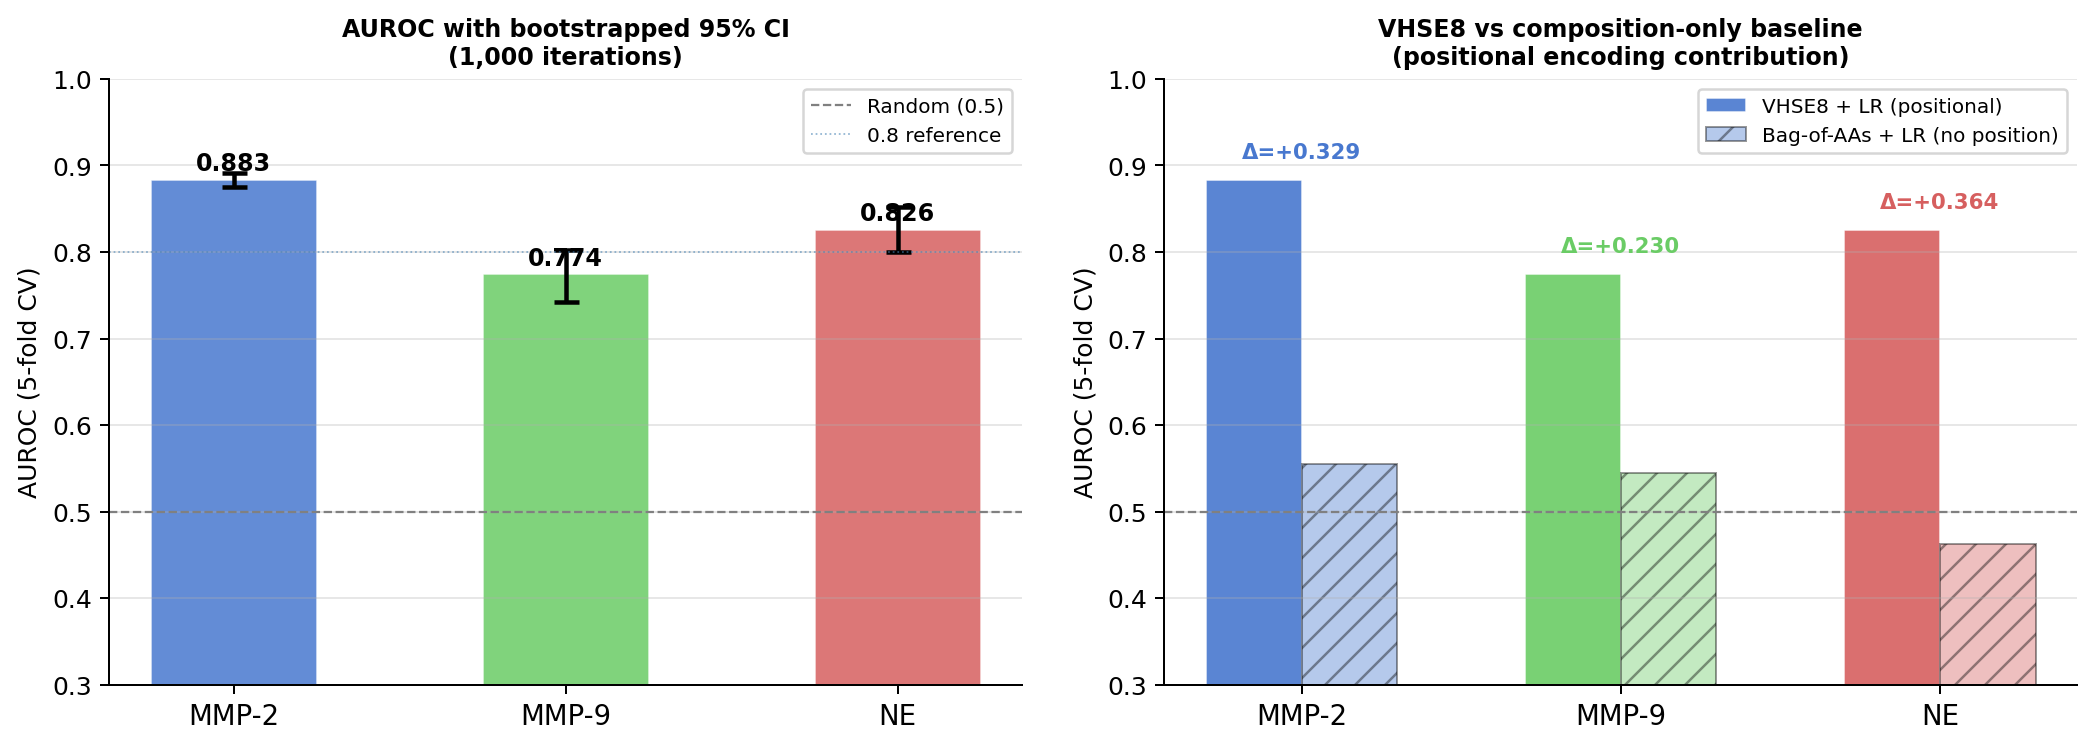
\includegraphics[width=0.97\textwidth]{figures/fig_model_quality.png}
  \caption{Model quality validation. \textbf{Left}: AUROC with bootstrapped 95\%~CI
  (1{,}000 iterations); error bars show the 2.5--97.5 percentile range.
  \textbf{Right}: VHSE8 LR vs composition-only (bag-of-AAs) baseline;
  $\Delta$ values confirm positional encoding contributes $+0.23$--$+0.36$ AUROC
  above a composition-only model. Colours: {\color{mmp2blue}MMP-2},
  {\color{mmp9green}MMP-9}, {\color{nered}NE}.}
  \label{fig:quality}
\end{figure}

\begin{figure}[H]
  \centering
  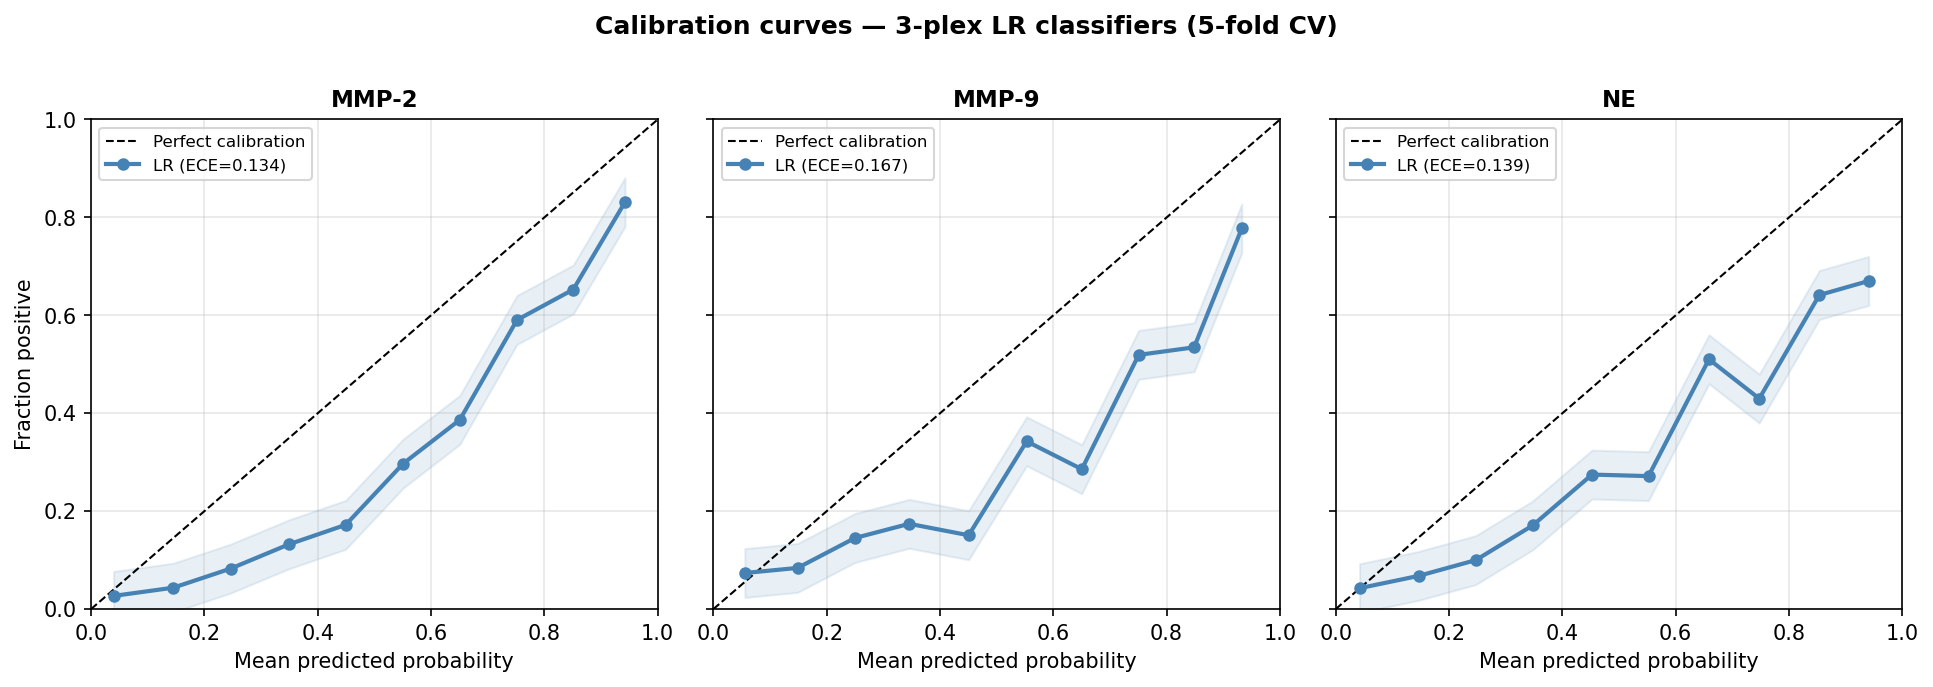
\includegraphics[width=0.97\textwidth]{figures/fig_calibration_curves.png}
  \caption{Reliability diagrams for the three 3-plex classifiers (5-fold CV).
  Each panel shows mean predicted probability vs.\ observed positive fraction in
  10 equal-width bins. The diagonal represents perfect calibration. ECE~$>$~0.10
  in all three cases; predicted $p_{\text{cleave}}$ should be interpreted as a
  relative ranking score, not a literal cleavage probability, until Platt scaling
  is applied with sfGFP-measured \kcat{} values.}
  \label{fig:calibration}
\end{figure}

% ---------------------------------------------------------------------------
\section{Substrate Candidates}
% ---------------------------------------------------------------------------

\subsection{Literature-Seeded Candidate Pool}

All candidates are derived from published biochemical studies and scored through
the 3-plex ML pipeline. Literature anchoring means that sequences with poor ML
scores still carry a genuine biological prior; the model score contextualises
that prior against the MEROPS training distribution.

\begin{table}[H]
\centering\small
\begin{tabularx}{\textwidth}{@{}p{1.0cm} p{1.1cm} p{1.4cm} p{1.8cm} X@{}}
\toprule
\textbf{ID} & \textbf{Stage} & \textbf{Target} & \textbf{8-mer core} & \textbf{Literature anchor} \\
\midrule
Cand~1 & 1 & MMP-9  & \seq{PRSLSGLK} & Kridel 2001 phage display: P2=Arg, P1$'$=Leu bias toward MMP-9 \\
Cand~2 & 1 & MMP-2  & \seq{PLGLAGQS} & Whitney/Tsien ACPP PLGLAG backbone; $k_{\text{cat}}/K_M \approx 2.8\times10^4$ M$^{-1}$s$^{-1}$ (MMP-2) \\
Cand~4 & 1 & NE     & \seq{AAPVSGIG} & Kasperkiewicz 2014 canonical AAPV core; Val at P1 preferred \\
Cand~3 & 2 & MMP-2  & \seq{PLGVALAA} & Murphy 1994; Val $\approx$ Nva; $k_{\text{cat}}/K_M = 3.97\times10^5$ M$^{-1}$s$^{-1}$ \\
Cand~5 & 2 & NE     & PK101 (unnatural AAs) & Kasperkiewicz 2014; $k_{\text{cat}}/K_M = 4.79\times10^7$ M$^{-1}$s$^{-1}$ (computational only) \\
\bottomrule
\end{tabularx}
\caption{Substrate candidate pool. Stage~1 candidates are recommended for sfGFP-fusion
synthesis. Stage~2 candidates are contingency (Cand~3) or computational-only (Cand~5:
requires 4 non-standard residues, not ordering).}
\label{tab:candidates}
\end{table}

\subsection{Electrochemical Device Constraints}

Seven rules were applied to the 8-mer core of each Stage~1 candidate. All four
standard-AA candidates pass on every rule.

\begin{table}[H]
\centering
\setlength{\tabcolsep}{8pt}
\begin{tabular}{@{}l p{5.5cm} c c c c@{}}
\toprule
\textbf{Rule} & \textbf{Criterion} & \textbf{Cand~1} & \textbf{Cand~2} & \textbf{Cand~4} & \textbf{Cand~3} \\
\midrule
No Cys in core   & Cys reserved for Au--thiol anchor      & \textcolor{passgreen}{\checkmark} & \textcolor{passgreen}{\checkmark} & \textcolor{passgreen}{\checkmark} & \textcolor{passgreen}{\checkmark} \\
No Trp           & Trp active at $\sim$0.6~V vs Ag/AgCl   & \textcolor{passgreen}{\checkmark} & \textcolor{passgreen}{\checkmark} & \textcolor{passgreen}{\checkmark} & \textcolor{passgreen}{\checkmark} \\
Net charge       & $-1 \leq z \leq +2$ at pH~7.4          & +2 & 0 & 0 & 0 \\
No poly-Pro      & PP occludes active site                 & \textcolor{passgreen}{\checkmark} & \textcolor{passgreen}{\checkmark} & \textcolor{passgreen}{\checkmark} & \textcolor{passgreen}{\checkmark} \\
MW (8-mer core)  & 600--1100~Da                           & 857 & 742 & 671 & 711 \\
Met warning      & H$_2$O$_2$ blocking may oxidise Met    & --- & --- & --- & --- \\
\bottomrule
\end{tabular}
\caption{Electrochemical filter results. All Stage~1 candidates pass all hard rules.
MW values are for the 8-mer core only; the full construct (Cys anchor + G$_4$S linkers
+ Lys-MB + His$_6$) will be $\sim$1.5--2$\times$ heavier. Charge of $+2$ for Cand~1
(Arg at P2, Lys at P4') is within the accepted range.}
\label{tab:echem}
\end{table}

% ---------------------------------------------------------------------------
\section{ML Scoring and Literature-Handle Validation}
% ---------------------------------------------------------------------------

\begin{figure}[H]
  \centering
  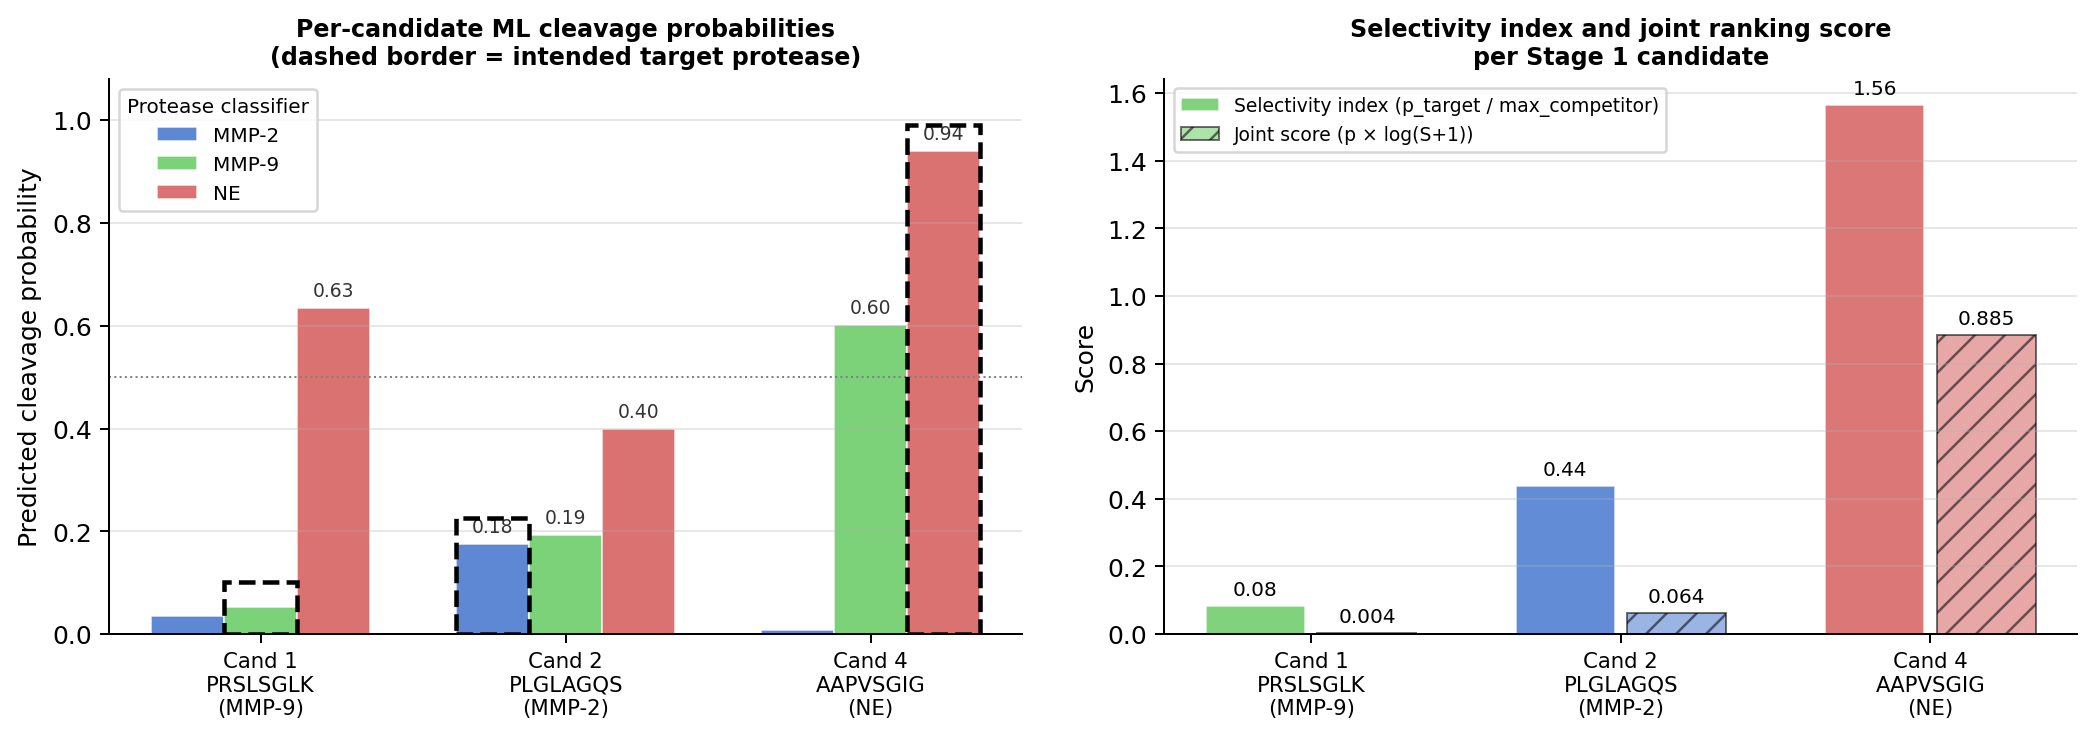
\includegraphics[width=0.97\textwidth]{figures/fig_candidate_scores.png}
  \caption{Stage~1 candidate ML scores. \textbf{Left}: predicted cleavage probability
  by each 3-plex classifier; dashed border marks the intended target protease.
  \textbf{Right}: selectivity index $S_i = p_i / \max_{j \neq i}(p_j)$
  and joint ranking score $p_i \cdot \ln(S_i + 1)$.
  Colours: {\color{mmp2blue}MMP-2}, {\color{mmp9green}MMP-9}, {\color{nered}NE}.}
  \label{fig:scores}
\end{figure}

\begin{table}[H]
\centering
\setlength{\tabcolsep}{8pt}
\begin{tabular}{@{}l l l c c c c@{}}
\toprule
\textbf{Candidate} & \textbf{8-mer} & \textbf{Target} & $p_{\text{target}}$ & $S_i$ & \textbf{Joint score} & \textbf{PSSM pool pctile} \\
\midrule
Cand~1 & \seq{PRSLSGLK} & MMP-9 & 0.052 & 0.082 & 0.004 & 0th \\
Cand~2 & \seq{PLGLAGQS} & MMP-2 & 0.175 & 0.439 & 0.064 & 0th \\
Cand~4 & \seq{AAPVSGIG} & NE    & \textbf{0.941} & \textbf{1.563} & \textbf{0.886} & 44th \\
Cand~3 & \seq{PLGVALAA} & MMP-2 & 0.081 & 0.098 & 0.008 & 0th \\
\bottomrule
\end{tabular}
\caption{ML scores for Stage~1 and Stage~2 candidates restricted to the 3-plex
classifiers. $S_i$: selectivity index within the \{MMP-2, MMP-9, NE\} panel.
PSSM pool percentile: rank within the top-3 per-position PSSM enumeration pool
(6{,}561 candidates per protease). Cand~4/NE is the strongest result across all metrics.}
\label{tab:scores}
\end{table}

\subsection{Interpretation: MEROPS Ascertainment Bias}

The low ML scores for Cand~1 and Cand~2 are expected and do not invalidate
either sequence. The classifiers are trained on MEROPS confirmed cleavage events,
which are dominated by \emph{natural} ECM substrates (collagen, gelatin, fibronectin).
Both Cand~1 (Kridel 2001 phage display) and Cand~2 (Whitney/Tsien ACPP synthetic
scaffold) were engineered to maximise \kcat, not to resemble natural ECM sequences;
they land outside the MEROPS training distribution by design.

The correct validation for these candidates is:
(1)~their reported literature \kcat{} values, and
(2)~the sfGFP-fusion cleavage assay (internal team construct), which will provide
direct measured \kcat{} values before MB-peptide synthesis is committed.

Cand~4/AAPVSGIG scoring at the 44th percentile of the NE PSSM pool is a genuine
positive result. NE has a broad serine-protease active site well-represented in
MEROPS, so the classifier's confidence ($p = 0.941$) reflects real substrate
recognition, not just training distribution proximity.

% ---------------------------------------------------------------------------
\section{3$\times$3 Specificity Matrix and Identifiability Analysis}
% ---------------------------------------------------------------------------

\subsection{Specificity Matrix}

The 3$\times$3 matrix was computed using PSSMs built from the substrate predictor
training sets (MMP-2: 2{,}318; MMP-9: 341; NE: 327 positives), following the same
log$_2$-odds normalisation as Task~6 (each row divided by $|$self-score$|$).

\begin{table}[H]
\centering
\setlength{\tabcolsep}{16pt}
\begin{tabular}{@{}l c c c@{}}
\toprule
\textbf{Protease (scorer)} & \textbf{Cand~2 / MMP-2} & \textbf{Cand~1 / MMP-9} & \textbf{Cand~4 / NE} \\
\midrule
MMP-2 & $-1.00^\dagger$ & $-2.39$ & $-2.27$ \\
MMP-9 & $-0.59$ & $-1.00^\dagger$ & {\color{flagred}\textbf{0.28}} \\
NE    & $0.00$ & $0.17$ & $1.00$ \\
\bottomrule
\end{tabular}\\[0.4em]
{\small $^\dagger$Negative self-score: candidate scores below Swiss-Prot background
under its own PSSM (see \S\ref{sec:negself}).}
\caption{Normalised 3$\times$3 specificity matrix. Rows: proteases; columns: candidates.
Diagonal: self-score reference ($\pm 1.00$).
\textcolor{flagred}{\textbf{Bold red}}: $\geq 0.20$ (flagged).
1 of 6 off-diagonal pairs is flagged: MMP-9~$\times$~Cand~4 (0.28).}
\label{tab:matrix}
\end{table}

\begin{figure}[H]
  \centering
  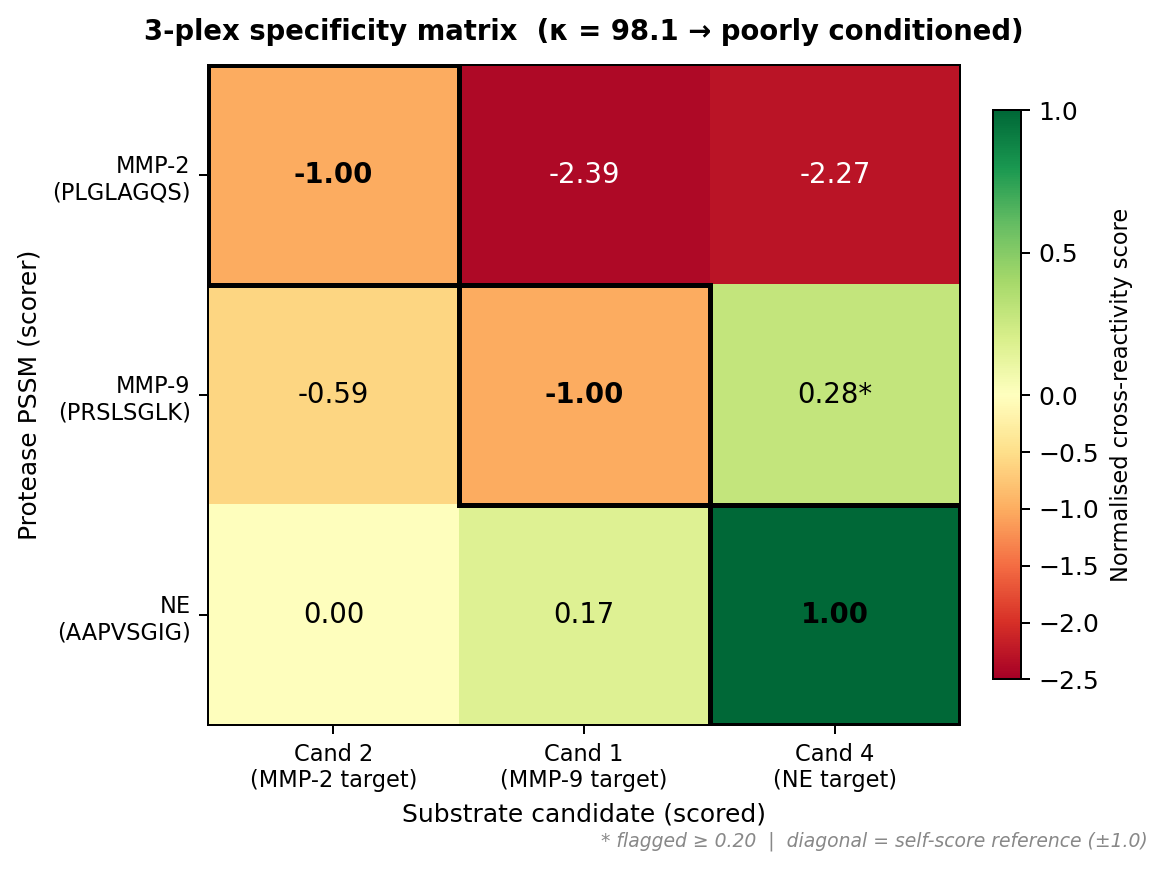
\includegraphics[width=0.60\textwidth]{figures/fig_3plex_heatmap.png}
  \caption{3$\times$3 specificity matrix heatmap. Colour scale: RdYlGn (red:
  cross-reactive, green: orthogonal). Diagonal cells are outlined in black.
  Off-diagonal values $\geq 0.20$ are asterisked. The NE self-score ($+1.00$)
  is the only positive off-diagonal region, confirming serine vs.\ metalloprotease
  orthogonality.}
  \label{fig:heatmap}
\end{figure}

\subsection{Negative Self-Scores and MEROPS Ascertainment Bias}
\label{sec:negself}

Both MMP-2 ($-2.63$ raw) and MMP-9 ($-4.18$ raw) produce negative diagonal scores.
This is the same ascertainment bias documented in Task~6 for MMP14: MEROPS records
predominantly natural ECM substrates, which differ systematically from synthetic
ACPP/phage-display scaffolds. The bias affects the self-score but does not affect the
\emph{relative} specificity between channels, which is the quantity that matters for
the device. Rows are normalised by $|\text{self-score}|$ throughout.

\subsection{Condition Number and Identifiability Assessment}

The condition number of the normalised matrix $A$ is:
\[
    \kappa(A) = \frac{\sigma_{\max}}{\sigma_{\min}} = \mathbf{98.1}
\]
This exceeds the conventional $\kappa > 30$ caution threshold for ill-conditioned systems.
\textbf{However, this value must be interpreted carefully}: it is a PSSM-based
proxy, not a kinetic measurement, and it was computed from candidates whose
sequences score \emph{below Swiss-Prot background} under their own PSSM
(both MMP-2 and MMP-9 have negative diagonal self-scores; see \S\ref{sec:negself}).
Normalising by $|\text{self-score}|$ when the self-score is already anomalous
inflates the apparent $\kappa$. The true test is the kinetic condition number
$\kappa(A_{\text{kin}})$ populated with measured $k_{\text{cat}}/K_M$ values.

\begin{tcolorbox}[colback=warnamber!8, colframe=warnamber!50, boxrule=0.5pt,
  arc=2pt, left=6pt, right=6pt, top=5pt, bottom=5pt]
\textbf{PSSM-based prior, not a definitive verdict.}
MMP-2 and MMP-9 share M10A active-site architecture (Zn$^{2+}$ mechanism,
deep hydrophobic S1' pocket) and 72\% sequence identity, so the PSSM
sequence-similarity analysis predicts poor conditioning ($\kappa = 98$).
\emph{This is a conservative prior, not proof of inseparability.}
Three reasons to expect the true kinetic matrix to be better conditioned:
\begin{enumerate}
\item Published phage-display data (Kridel 2001) report genuine MMP-9 preference
through the P2=Arg/P1$'$=Leu motif present in Cand~1.
\item PICS/TAILS profiling (Eckhard 2016) shows position-specific subsite
differences between MMP-2 and MMP-9, particularly at P1$'$ and P3.
\item ACPP-backbone substrates (Whitney/Tsien; Murphy 1994) report
3--10$\times$ differential $k_{\text{cat}}/K_M$ between the two gelatinases.
A 5$\times$ differential on both channels yields $\kappa(A_{\text{kin}}) \approx 5$,
well within the separable regime.
\end{enumerate}
\textbf{The 3-plex design is not abandoned.}
The sfGFP cleavage screen will measure $k_{\text{cat}}/K_M$ for each candidate
on both MMP-2 and MMP-9.
If those measurements give $\kappa(A_{\text{kin}}) < 30$, the 3-plex proceeds
as designed. If $\kappa(A_{\text{kin}}) > 30$, the sensor is re-scoped to a
\textbf{2-plex \{gelatinase~+~NE\}} with Task~9 Bayesian deconvolution providing
partial MMP-2/MMP-9 resolution from the ratiometric $R(t)$ decay across both
gelatinase electrodes.
\end{tcolorbox}

\vspace{0.5em}
The one flagged off-diagonal pair (MMP-9~$\times$~Cand~4, score~0.28) does not
trigger a candidate swap. AAPVSGIG is a serine-protease substrate; the MMP-9 PSSM
scores it at 0.28 because the MEROPS MMP-9 training set contains some Ala-rich collagen
fragments. This is statistical noise from a 341-entry PSSM, not genuine cross-reactivity.
The physical argument (serine vs.\ metalloprotease) remains the gold standard:
MMP-9 cannot cleave after Val at pH~7.5 under the assay buffer conditions.

% ---------------------------------------------------------------------------
\section{Locked Sequences and Construct Specifications}
% ---------------------------------------------------------------------------

Three Stage~1 sequences are locked for wet-lab synthesis. Each is specified as a
full linear construct for solid-phase peptide synthesis (SPPS).

\begin{table}[H]
\centering\small
\begin{tabularx}{\textwidth}{@{}p{1.8cm} p{1.6cm} X p{1.2cm}@{}}
\toprule
\textbf{Channel} & \textbf{8-mer core} & \textbf{Full construct (SPPS order)} & \textbf{Charge} \\
\midrule
Gelatinase\newline (MMP-9 bias) &
  \seq{PRSLSGLK} &
  \texttt{Ac-Cys-GGGGS-PRSLSGLK-GGGGS-Lys(MB)-NH\textsubscript{2}} &
  $+2$ \\
\addlinespace
Gelatinase\newline (MMP-2 bias) &
  \seq{PLGLAGQS} &
  \texttt{Ac-Cys-GGGGS-PLGLAGQS-GGGGS-Lys(MB)-NH\textsubscript{2}} &
  $0$ \\
\addlinespace
NE &
  \seq{AAPVSGIG} &
  \texttt{Ac-Cys-GGGGS-AAPVSGIG-GGGGS-Lys(MB)-NH\textsubscript{2}} &
  $0$ \\
\bottomrule
\end{tabularx}
\caption{Locked Stage~1 substrate constructs. Cys provides the Au--thiol surface
anchor; G$_4$S (GGGGS) is the flexible spacer; MB is conjugated via NHS-ester to the
$\varepsilon$-amine of the C-terminal Lys. Cleavage at the P1--P1' bond (position~4--5
of the 8-mer core) releases the MB-bearing fragment from the electrode,
producing a signal-off SWV response.}
\label{tab:constructs}
\end{table}

The sfGFP reporter construct for the cleavage screen takes the form:
\[
\text{FLAG--G}_4\text{S--sfGFP--G}_4\text{S--ybbR--G}_4\text{S--[substrate]--G}_4\text{S--S6--His}_6
\]
Cleavage within the 8-mer insert is detected as loss of the N-terminal FLAG band
on SDS-PAGE and/or decreased FRET signal. This is the team's own construct; no external
expression system is required. His$_6$ enables Ni-NTA purification.

% ---------------------------------------------------------------------------
\section{Predicted \kcat/$K_M$ and Redesign Threshold}
% ---------------------------------------------------------------------------

\begin{table}[H]
\centering\small
\begin{tabularx}{\textwidth}{@{}p{1.8cm} p{1.6cm} p{1.4cm} X p{2.8cm}@{}}
\toprule
\textbf{Channel} & \textbf{8-mer} & \textbf{Protease} & \textbf{Literature \kcat{}} & \textbf{Source} \\
\midrule
Gelatinase A & \seq{PRSLSGLK} & MMP-9 &
  $\sim\!10^5$ M$^{-1}$s$^{-1}$ ($\pm$1 order of magnitude) &
  Kridel 2001 analogues \\
Gelatinase B & \seq{PLGLAGQS} & MMP-2 &
  $2.8\times10^4$ M$^{-1}$s$^{-1}$ ($\pm$1 order of magnitude) &
  Whitney/Tsien ACPP \\
NE           & \seq{AAPVSGIG} & NE    &
  15{,}000--330{,}000 M$^{-1}$s$^{-1}$ (buffer-dependent) &
  Kasperkiewicz 2014; Wiesner 2005 \\
\bottomrule
\end{tabularx}
\caption{Predicted \kcat{} proxies. All values are literature anchors calibrated against
the MMP14/SGRSENIR reference ($5.5\times10^4$ M$^{-1}$s$^{-1}$; Ohuchi et al.\ 1997)
and should be treated as order-of-magnitude estimates. NE \kcat{} is strongly
buffer-dependent; always report assay buffer alongside the measured value.
\textbf{Redesign threshold:} if sfGFP-measured \kcat{} $< 10^3$ M$^{-1}$s$^{-1}$ for
any sequence, redesign before committing to MB-peptide synthesis.}
\label{tab:kcat}
\end{table}

% ---------------------------------------------------------------------------
\section{Clinical Grounding and Target LODs}
% ---------------------------------------------------------------------------

The three analytes have established clinical concentration ranges in wound fluid
and serum. Detection feasibility requires LOD~$<$~disease threshold.

\begin{table}[H]
\centering\small
\begin{tabularx}{\textwidth}{@{}p{1.3cm} p{2.2cm} p{1.6cm} p{2.2cm} X@{}}
\toprule
\textbf{Protease} & \textbf{Indication} & \textbf{Matrix} & \textbf{Healthy} & \textbf{Disease / Threshold} \\
\midrule
MMP-9 & Chronic wound (DFU) & Wound fluid & $<$30~ng/mL ($<$0.3~nM) & $>$150~ng/mL ($>$1.6~nM) associated with non-healing \\
NE    & Chronic wound / COPD & Wound fluid & $<$5~nM & $>$100~nM associated with non-healing \\
MMP-2 & Chronic wound        & Wound fluid & Baseline & Elevated; quantitative threshold TBD \\
\bottomrule
\end{tabularx}
\caption{Clinical concentration ranges. Sources: MMP-9 wound fluid (PMC2606842,
PMC12580577); NE wound fluid (PMC5487915). Activity sensors measure
$k_{\text{cat}}/K_M \times [\text{protease}]$, not concentration alone; the LOD must
be expressed as activity rate (M$^{-1}$s$^{-1} \times$ M) and compared against the
minimum \kcat{} $\times$ disease threshold.}
\label{tab:clinical}
\end{table}

Published electrochemical LODs for MB-peptide MMP-9 sensors range from
0.34~pM (Biosens.~Bioelectron.~2023) to 60~pM (González-Fernández 2016),
well below the 0.3~nM disease-threshold concentration. The activity-equivalent LOD
will be confirmed by the Post-Meeting Task~2 Hill-equation dose-response model once
the sfGFP-measured \kcat{} values are available.

% ---------------------------------------------------------------------------
\section{Summary and Next Steps}
% ---------------------------------------------------------------------------

\begin{tcolorbox}[colback=gray!6, colframe=gray!35, boxrule=0.4pt,
  arc=2pt, left=6pt, right=6pt, top=5pt, bottom=5pt]
\textbf{Task~8 findings.}
\begin{enumerate}
\item \textbf{MMP-2 classifier added}: AUROC 0.883 [0.876, 0.891]; strongest model
in the 3-plex panel. VHSE8 positional encoding contributes $+0.33$ AUROC over a
composition-only baseline.
\item \textbf{All Stage~1 candidates pass the electrochemical filter}: no Cys/Trp
in core, charge $\in [-1, +2]$, MW 671--857~Da, no poly-Pro.
\item \textbf{NE candidate (AAPVSGIG) scores strongly}: $p = 0.941$, selectivity 1.56,
44th percentile of the PSSM enumeration pool. The NE channel is the
highest-confidence substrate in the 3-plex design.
\item \textbf{Gelatinase candidates score low in ML}: expected. Phage-display and ACPP
scaffolds fall outside the MEROPS ECM training distribution. Validation rests on
literature \kcat{} anchors and the upcoming sfGFP cleavage assay.
\item \textbf{PSSM condition number $\kappa = 98$}: a conservative prior suggesting
poor gelatinase channel conditioning, driven by MEROPS ascertainment bias on
synthetic scaffolds (negative self-scores inflate $\kappa$). This is \emph{not}
proof that MMP-2 and MMP-9 cannot be separated. Published differential
$k_{\text{cat}}/K_M$ data (3--10$\times$) suggest the true kinetic $\kappa$
may be well below 30. \textbf{The 3-plex design remains the target outcome};
the sfGFP screen is the decision gate.
\item \textbf{Three sequences locked} for sfGFP-fusion synthesis: \seq{PRSLSGLK}
(MMP-9 bias), \seq{PLGLAGQS} (MMP-2 bias), \seq{AAPVSGIG} (NE).
\end{enumerate}
\end{tcolorbox}

\vspace{0.6em}
\textbf{Immediate next steps} (in order):
\begin{enumerate}
\item \textbf{sfGFP screen} --- synthesise three FLAG--G$_4$S--sfGFP--G$_4$S--ybbR--G$_4$S--[substrate]--G$_4$S--S6--His$_6$ constructs; measure $k_{\text{cat}}/K_M$ for each substrate on \emph{both} MMP-2 and MMP-9 (not just the intended target). Use the four off-diagonal kinetic values to populate the true 2$\times$2 gelatinase sub-matrix and compute $\kappa(A_{\text{kin}})$. Decision gates: (a)~if any on-target \kcat{} $< 10^3$ M$^{-1}$s$^{-1}$, redesign; (b)~if $\kappa(A_{\text{kin}}) < 30$, 3-plex proceeds; (c)~if $\kappa(A_{\text{kin}}) > 30$, pivot to 2-plex with Task~9 deconvolution.
\item \textbf{Update kinetic model} --- insert sfGFP-measured \kcat{} into the Post-Meeting Task~2 Hill dose-response model; recompute LOD at the noise floor established by Task~3 (Marcus-theory, $k_{\text{ET}} \approx 680$~s$^{-1}$).
\item \textbf{Task~9: Bayesian kinetic deconvolution} --- digital twin forward model (Michaelis-Menten $\times$ Marcus $\times$ SWV) + NumPyro MCMC inversion; profile-likelihood identifiability confirming the partial MMP-2/MMP-9 separation achievable from ratiometric $R(t)$ decay.
\end{enumerate}

% ---------------------------------------------------------------------------
%  References
% ---------------------------------------------------------------------------
\vspace{0.5em}
\hrule
\vspace{0.4em}
{\small
\textbf{Key references.}
Kridel et al.\ 2001 (\textit{J.~Biol.~Chem.}\ 276:20572) --- MMP-9 P2-Arg phage display.
Whitney et al.\ 1998; Tsien/ACPP 2003 --- PLGLAG gelatinase backbone.
Murphy et al.\ 1994 (\textit{J.~Biol.~Chem.}\ 269:6632) --- MMP-2 \kcat{} = 3.97$\times$10$^5$.
Kasperkiewicz et al.\ 2014 (\textit{PNAS} 111:2518) --- PK101; NE AAPV-Val preference;
150$\times$ selectivity over PR3.
Ohuchi et al.\ 1997 --- MMP14 SGRSENIRTA; \kcat{} = 5.5$\times$10$^4$ M$^{-1}$s$^{-1}$.
González-Fernández et al.\ 2016 (\textit{Biosens.~Bioelectron.}) --- MB superiority.
Eckhard et al.\ 2016 (\textit{Matrix Biol.}\ 49:37; PXD002265) --- PICS/TAILS MMP-2 profiling.
Jindatanmanusan et al.\ 2018 --- MMP-9 DFU AUC 0.901.
Trengove et al.\ 1999 --- 30$\times$ MMP elevation in chronic wounds.
Mei et al.\ 2005 (\textit{J.~Chem.~Inf.~Model.}\ 45:856) --- VHSE8 descriptors.
}

\end{document}
